\documentclass[11pt]{article}

\usepackage{amsmath, amsfonts, amssymb, graphicx, soul, parskip, cancel}

\newcommand{\independent}[0]{\perp\!\!\!\perp}

\setlength{\parindent}{0pt} 

\begin{document}

\begin{center}\ul{Errata to Chalk-Talk, 10/21/2024:} \\
Identification of Some but Not All Strategies 
\end{center}
\vspace{.25in}

Recall:  We were asking how it is that we can see that $\mathbb E[Y^{a_0,
a_1}]$ is identified in Figure 19.8 but not 19.10.

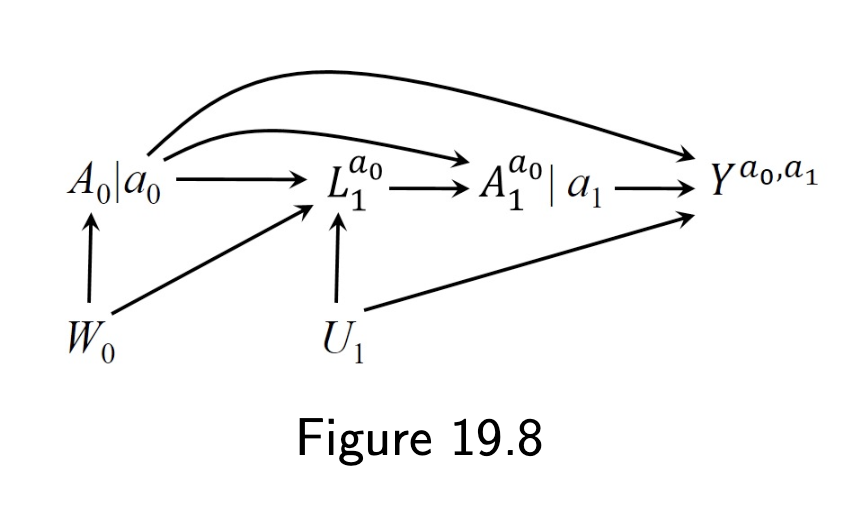
\includegraphics[width=2.5in]{fig198.png}
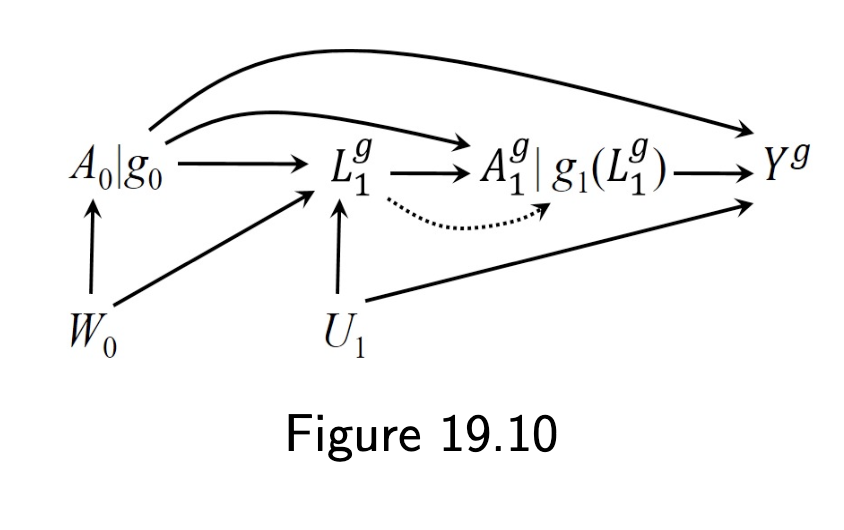
\includegraphics[width=2.25in]{fig1910.png}

The statement of sequential randomization $Y^{\bar{a}} \independent A_k | \bar{A}_{k-1}, \bar{L}_{k}$ can be 
interpreted as saying that if we want to be able to identify $\mathbb E[Y^{\bar{a}}]$ 
then we should be able to confirm that $Y^{\bar{a}}$ and $A_k$ are d-separated
given the appropriate conditioning set. 

In the case where $\bar{A}_k = (A_0, A_1)$, then the conditional independences we need to check 
are 
\begin{itemize}
\item $Y^{a_0, a_1} \independent A_0 | L_0$, and 
\item $Y^{a_0, a_1} \independent A_1 | A_0, L_0, L_1.$ 
\end{itemize}

In Figures 19.8 and 19.10, the simplifying assumption that $L_0$ does not exist is made. 

Make particular note that sequential randomization implies an unconditional independence for 
$Y^{a_0, a_1}$ and $A_0$ when $L_0$ does not exist. 

If you refer to Figure 19.8, we can see the following: 

\begin{itemize}
\item If we are checking if $Y^{a_0, a_1}$ and $A_0$ satisfy the criteria for sequential exchangeability (e.g., are conditionally independent given the right conditioning set), 
the following path is blocked: $Y^{a_0, a_1} \leftarrow U_1 \rightarrow
L_1^{a_0} \leftarrow W_0 \rightarrow A_0$.  The reason it is blocked is that
$L_1$ is a collider on this path, and $L_1$ is not being conditioned on (recall
the conditioning set for $A_0$ to check sequential randomization is just $L_0$,
assumed not to exist in this example). 
\item If we are checking if $Y^{a_0, a_1}$ and $A_1$ are conditionally independent given $\{ A_0, L_1 \}$, 
then observe that the following path is blocked: $Y^{a_0, a_1} \leftarrow U_1 \rightarrow \boxed{L_1^{a_0}} \rightarrow A_1^{a_0}$. Here, $L_1$ is a normal node (not a collider on this path) but it is conditioned on, so it blocks the path. 
\item There are a couple other paths connecting $Y^{a_0, a_1}$ and $A_0, A_1$ but these are 
easily confirmed to be blocked because along them are non-colliders being conditioned on.
\end{itemize}

This confirms that $\mathbb E[Y^{a_0, a_1}]$ is identified under the SWIG of 19.8 which represents 
a static treatment regime even in the presence of $W_0$, an unobserved confounder of treatment and
measured covariate $L_1^{a_0}$. 

Now consider what happens when we consider a dynamic regime, as in Fig 19.10. 
Then look and see if there is an open path between $A_0$ and $Y^g$.  Indeed there is. 
The statement of conditional randomization as it applies to $Y^g$ and $A_0$ says 
that we should check if $Y^g \independent A_0 | L_0$, and the only element of the conditioning set 
is $L_0$, which doesn't exist in these SWIGs. As a result, we only need to check 
if $A_0$ and $Y^g$ are independent, or in other words, d-separated given the
empty conditioning set $\varnothing = \{ \}$. Observe this path is open: $A_0
\leftarrow W_0 \rightarrow L_1^g \rightarrow g_1(L_1^g) \rightarrow Y^g$. Of
course this path is open, because we do not condition on future events $L_1^g$
or $g_1(L_1^g)$ as part of checking the sequential exchangeability criterion as
it applies to $Y^g$ and $A_0$. None of the nodes in this path are conditioned on,
nor are they colliders, so the path is open by the definition of d-separation we covered yesterday. 

This concludes the demonstration that the mean counterfactual outcomes under a dynamic treatment regime 
cannot be identified in the presence of $W_0$ if the data are correctly represented by SWIG/Fig 19.10.

As a result, we conclude that there is a DAG we can draw (Fig 19.6) (consistent
with both SWIGS Fig 19.8 and 19.10) under which only static treatment regimes
have mean counterfactual outcomes identified while dynamic treatment regimes do
not. \hfill $\divideontimes$

\begin{center}
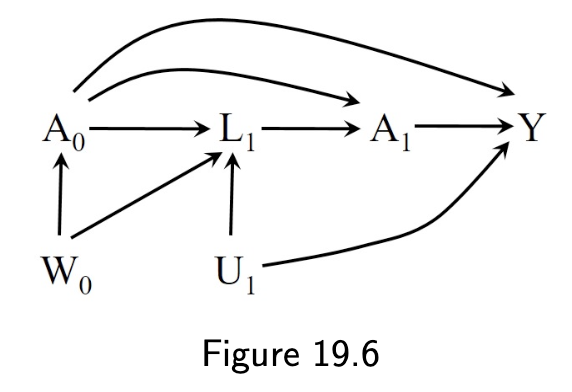
\includegraphics[width=2in]{fig196.png}
\end{center}
\end{document}
